\documentclass{article}
\usepackage[utf8]{inputenc}

\usepackage{depreequantum}

\title{Quantum Homework Template}
\author{Erin De Pree}
\date{Fall 2019}

\usepackage{natbib}
\usepackage{graphicx}

\begin{document}

\maketitle

\section*{Suppressing Section Numbering}
    If you are going to label your sections by problem number, then it is a good idea to use \verb+\section*+ instead of \verb+\section+ so you can suppress the section numbering.  This way you won't  write ``3 Problem 2''!
    
    Here, I'm going to work through problem 1.5 from our text.  This will show you how to write kets and such.  I've also included a section on matrices so you can see how to write them up.
    
    Be sure to include the \verb+depreequantum.sty+ style file as it loads the necessary packages.
    
\section*{Problem 1.5}
	A beam of spin-1/2 particles is prepared in the state
	\[	\ket{\psi} = \tfrac{2}{\sqrt{13}} \ket{+} + i \tfrac{3}{\sqrt{13}} \ket{-}	\]
	
	\paragraph{Part a} What are the possible results of a measurement of the spin component $S_z$, and with probabilities would they occur?
	
		You will either measure $S_z = +\hbar/2$ (spin up) or $S_z = - \hbar/2$ (spin down).
		
		The probability of measuring $S_z = +\hbar/2$ is
		\begin{align*}
			\mathcal{P}_+ &= \abs{ \braket{+}{\psi} }^2 
			= \abs{ \bra{+} \qty( \frac{2}{\sqrt{13}} \ket{+} + i \frac{3}{\sqrt{13}} \ket{-} ) }^2 \\
			&= \abs{ \frac{2}{\sqrt{13}} \braket{+} + i \frac{3}{\sqrt{13}} \braket{+}{-} }^2\\
			&= \abs{ \frac{2}{\sqrt{13}} + 0 }^2 
			= \boxed{ \frac{4}{13} \simeq 31\% }
		\end{align*}
		While the probability of measuring $S_z = - \hbar/2$ is
		\begin{align*}
			\mathcal{P}_- &= \abs{ \braket{-}{\psi} }^2 
			= \abs{ \bra{-} \qty( \frac{2}{\sqrt{13}} \ket{+} + i \frac{3}{\sqrt{13}} \ket{-} ) }^2 \\
			&= \abs{ \frac{2}{\sqrt{13}} \braket{-}{+} + i \frac{3}{\sqrt{13}} \braket{-} }^2 \\
			&= \abs{ 0 + i \frac{3}{\sqrt{13}} }^2 
			= \qty( -i\frac{3}{\sqrt{13}} ) \qty( i \frac{3}{\sqrt{13}} ) \\
			&= -i^2 \frac{9}{13} 
			= \boxed{ \frac{9}{13} \simeq 69\% }
		\end{align*}
		
	\paragraph{Part b} What are the possible results of a measurement of the spin component $S_x$, and with probabilities would they occur?
		
		Measure $S_x = \pm \hbar/2$.
		
		Probability of measuring $S_x = +\hbar/2$ is
		\begin{align*}
			\mathcal{P}_{+x} &= \abs{ {}_x\braket{+}{\psi} }^2 
			= \abs{ \qty( \frac{1}{\sqrt{2}} \bra{+} +  \frac{1}{\sqrt{2}} \bra{-} ) \qty( \frac{2}{\sqrt{13}} \ket{+} + i \frac{3}{\sqrt{13}} \ket{-} ) }^2 \\
			&= \abs{ \frac{1}{\sqrt{2}} \frac{2}{\sqrt{13}} + i \frac{1}{\sqrt{2}} \frac{3}{\sqrt{13}} }^2 
			= \abs{ \frac{2 + 3i}{\sqrt{26}} }^2 \\
			&= \frac{1}{26} \qty( 2 - 3i ) \qty( 2+3i ) 
			= \frac{ 4 - 6i + 6i - 9i^2}{26} \\
			&= \frac{4 + 9}{26} 
			= \frac{13}{26} 
			= \boxed{ \frac{1}{2} = 50\% }
		\end{align*}
		Probability of measuring $S_x = -\hbar/2$ is
		\begin{align*}
			\mathcal{P}_{-x} &= \abs{ {}_x\braket{-}{\psi} }^2 
			= \abs{ \qty( \frac{1}{\sqrt{2}} \bra{+} -\frac{1}{\sqrt{2}} \bra{-} ) \qty( \frac{2}{\sqrt{13}} \ket{+} + i \frac{3}{\sqrt{13}} \ket{-} ) }^2 \\
			&= \abs{ \frac{1}{\sqrt{2}} \frac{2}{\sqrt{13}} - i \frac{1}{\sqrt{2}} \frac{3}{\sqrt{13}} }^2 
			= \abs{ \frac{2 - 3i}{\sqrt{26}} }^2 \\
			&= \frac{1}{26} \qty( 2 + 3i ) \qty( 2-3i ) 
			= \frac{ 4 - 6i + 6i - 9i^2}{26} \\
			&= \frac{4 + 9}{26} 
			= \frac{13}{26} 
			= \boxed{ \frac{1}{2} = 50\% }
		\end{align*}
		
	\paragraph{Part c}  Histograms!  See \cref{fig:HistrogramsProblem1.5} for the histograms.  Also note the figure appears on the next page because \LaTeX{} is automatically placing it where it makes most sense (after it is referenced).
		
		\begin{figure}
			\begin{center}
			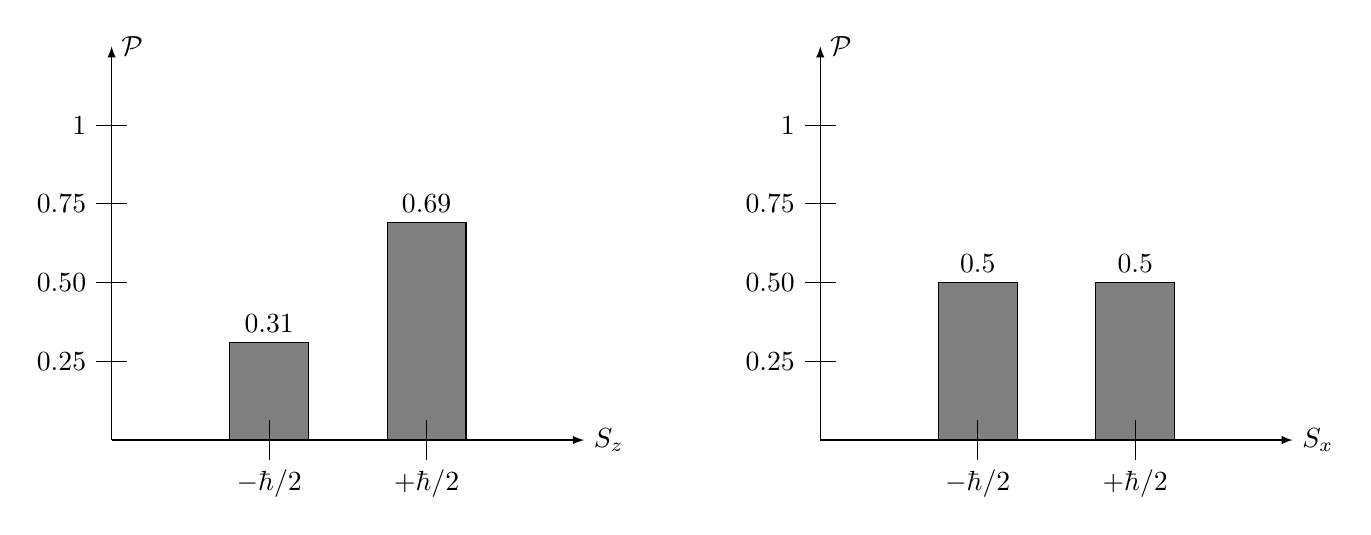
\begin{tikzpicture}[>=latex]
				\begin{scope}
					\draw[->]	(0,0) -- (6,0) node[right]{$S_z$};
					\draw[->]	(0,0) -- (0,5) node[right]{$\mathcal{P}$};
					\foreach \x / \spin / \prob in {2/-/0.31, 4/+/0.69}
					{	\draw[fill=Grey]	(\x,0) ++(-0.5, 0) rectangle ++(1,4*\prob) ++(-0.5,0) node[above]{$\prob$};
						\draw	(\x, -0.25) node[below]{$\spin \hbar/2$} -- ++(0, 0.5);
					}
					\foreach \y / \prob in {1/0.25, 2/0.50, 3/0.75, 4/1}
					{	\draw	(-0.2, \y) node[left]{$\prob$} -- ++(0.4,0);	}
				\end{scope}
				\begin{scope}[xshift=9cm]
					\draw[->]	(0,0) -- (6,0) node[right]{$S_x$};
					\draw[->]	(0,0) -- (0,5) node[right]{$\mathcal{P}$};
					\foreach \x / \spin / \prob in {2/-/0.5, 4/+/0.5}
					{	\draw[fill=Grey]	(\x,0) ++(-0.5, 0) rectangle ++(1,4*\prob) ++(-0.5,0) node[above]{$\prob$};
						\draw	(\x, -0.25) node[below]{$\spin \hbar/2$} -- ++(0, 0.5);
					}
					\foreach \y / \prob in {1/0.25, 2/0.50, 3/0.75, 4/1}
					{	\draw	(-0.2, \y) node[left]{$\prob$} -- ++(0.4,0);	}
				\end{scope}
			\end{tikzpicture}
			\end{center}
			
			\caption{Probabilities of measuring various spins in problem 1.5.  You may find it easier to make your histograms in Excel or Google Sheets or by hand and include them as a picture.}
			\label{fig:HistrogramsProblem1.5}
		\end{figure}


\section*{Matrix Notation}

	Going to use $\dot{=}$ to mean \emph{represented by}.  In \LaTeX\,, use the notation: \verb+\dot{=}+.  The quantum state isn't a column vector, but it can be represented by a column vector
	\begin{align}
		\ket{+} &\dot{=} \mqty( 1 \\ 0 ) 
		& \ket{-} &\dot{=} \mqty( 0 \\ 1) 
		\label{eq:basismatrix}
	\end{align}
	This is the $z$-basis set.
	
	Let's use the column vector notation to represent a state $\ket{\psi}$ as a projection of the state on the $\ket{+}$ and the projection on the $\ket{-}$:
	\[	\ket{\psi} \dot{=} \mqty( \braket{+}{\psi} \\ \braket{-}{\psi} )	\]
	
	\[	\ket{\psi} = a \ket{+} + b \ket{-}	\]
	
	\[	\ket{\psi} \dot{=} \mqty( a \\ b )	\]
	
	\[	\bra{\psi} \dot{=} \mqty( a^\ast & b^\ast )	\]
	
	We can also write the $x$ and $y$ kets in the $z$-basis:
	\begin{align*}
		\ket{+}_x &\dot{=} \frac{1}{\sqrt{2}} \mqty( 1 \\ 1) 
		& \ket{+}_y&\dot{=} \frac{1}{\sqrt{2}} \mqty( 1 \\ i ) \\
		\ket{-}_x &\dot{=} \frac{1}{\sqrt{2}} \mqty( 1 \\ -1 )
		& \ket{-}_y &\dot{=} \frac{1}{\sqrt{2}} \mqty( 1 \\ -i )
	\end{align*}

\end{document}